\documentclass[]{article}
\usepackage[hyphens]{url}
\usepackage[pdfusetitle,colorlinks,plainpages]{hyperref}
\usepackage[dutch]{babel}
\usepackage{lipsum} % for dummy text only
\usepackage{csquotes}
\usepackage[backend=bibtex]{biblatex}
%\usepackage[acronym]{glossaries}
\usepackage{eurosym}
\usepackage{subfigure}
\usepackage{multirow}
\usepackage{tikz}
\usepackage{listings}
\usepackage{caption}
\usepackage{pdfpages}

\usepackage{todonotes}
\usepackage{placeins}

\usepackage{tikz}
\usepackage{pgfplots}
\usepackage{verbatim}

%opening
\title{IMP: YCSB}
\author{Thomas Uyttendaele}

\begin{document}

\maketitle
\section{Algemene inleiding}
In deze sectie zal voor de verschillende systemen de automatisering van installatie en configuratie met behulp van IMP uitgelegd worden. Er zal steeds de afhankelijkheden gegeven worden, een domeinmodel, uitleg bij het domeinmodel en voorbeeld configuratie gegeven worden. 

De automatisatie van installatie is ontwikkeld en getest met Fedora 18 en 20, op andere distributies en versies is er niet getest. 
Elk systeem maakt gebruik van \textit{ip::services::Server}, een instantie hiervan is een (virtuele) machine met een IP adres en besturingssysteem. 

Bij elke instantie is het verplicht om de firewall uit te zetten en SELinux op permissive te zetten. Dit kan met behulp van de volgende commando's: 
\begin{lstlisting}[frame=single, breaklines=true]
systemctl stop firewalld.service  
systemctl disable firewalld.service  
setenforce 0
sed -i "s/SELINUX=enforcing/SELINUX=permissive/g" /etc/sysconfig/selinux
sed -i "s/SELINUX=enforcing/SELINUX=permissive/g" /etc/selinux/config|
\end{lstlisting}

\section{YCSB}
\textit{Link: \url{https://github.com/thuys/ycsb}}

Benodigde IMP modules: std, net, ip, redhat, hosts, yum, git, hbase, mongodb, pgpool-II 

De installatie en configuratie is gebeurd aan de hand van de uitleg van YCSB\footnote{\url {https://github.com/brianfrankcooper/YCSB/wiki/}}. 

\subsection{Domein model en uitleg}
Het domeinmodel is te zien in figuur \ref{fig:imp-ycsb-domeinmodel}.
\begin{figure}[ht!]
\centering
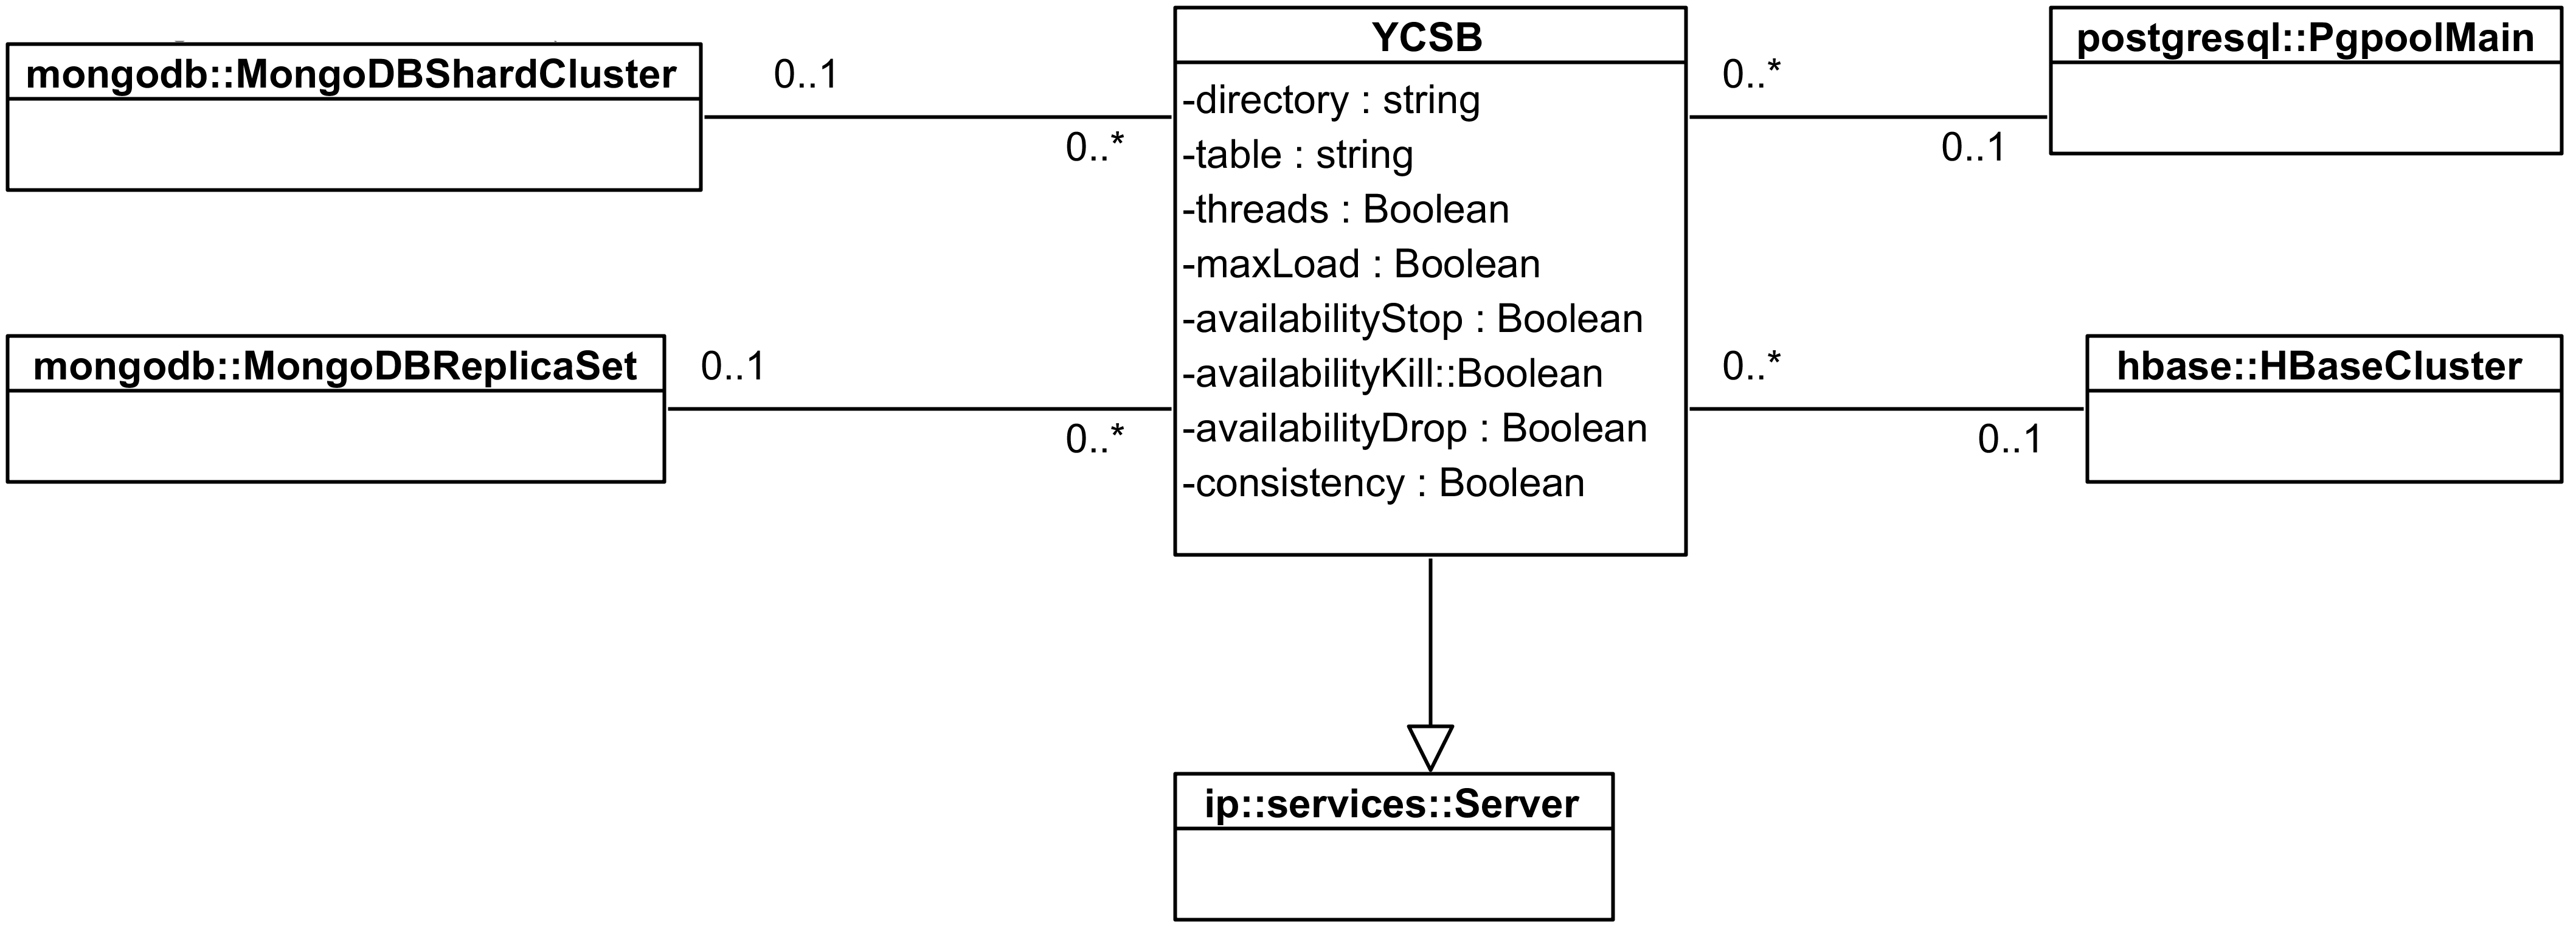
\includegraphics[width=\linewidth]{img/YCSB-Domeinmodel.png}
\caption{YCSB: Domeinmodel YCSB in IMP}
\label{fig:imp-ycsb-domeinmodel}
\end{figure}

Dit model bevat maar 1 nieuw element en dit is YCSB. Deze dient verbonden te zijn met één van de 3 systemen die hierboven zijn beschreven. Elk van deze systemen zal getest worden voor alle testen die geactiveerd zijn. MongoDB heeft 2 connecties omdat de cluster voor de beschikbaarheidstesten wordt gebruikt en een replicaset voor de consistentie testen. Pgpool-II heeft geen ondersteuning voor de consistentie testen. 

\subsection{Voorbeeld configuratie}

De configuratie voor de testomgeving gaat als volgt in IMP: 

\lstinputlisting[language=Python, breaklines=true, frame=single]{code/imp-ycsb.conf}

De testen starten door het uitvoeren van {{directory}}/scripts/ycsb-script. De resultaten komen in de folder {{directory}}/results. 


\section{Uitvoeren testen}
Voor het uitvoeren van de testen dienen de besproken systemen online gebracht te worden, met op het minst YCSB en daarnaast 1 database systeem. 

In de installatie folder van YCSB bevindt zich de map \textit{scripts}. Om al de testen uit te voeren dient het bestand \textit{ycsb-script} van die folder uitgevoerd te worden. De configuratie van elke script kan aangepast worden in de map \textit{config} van YCSB. 

Als het script voltooid it, kan met behulp van de R-code (\url{https://github.com/thuys/YCSB-R-Scripts}) de grafieken gecreeërd worden. Dit gebeurt door het aanpassen en uitvoeren van \textit{Plot-consistentie.R} en \textit{Plot-calibratie-en-beschikbaarheid.R}. Belangrijk is om de \textit{basicDir} van beide scripts correct te zetten. 
\end{document}
